\documentclass[fleqn]{article}
\usepackage{course}
\setlength{\abovedisplayskip}{3pt}
\usepackage{mathtools}
\usepackage[T1]{fontenc}
\lstset{upquote=true}
 
\definecolor{dkgreen}{rgb}{0,0.6,0}
\definecolor{gray}{rgb}{0.5,0.5,0.5}
\definecolor{mauve}{rgb}{0.58,0,0.82}

\lstset{frame=tb,
  language=C,
  aboveskip=3mm,
  belowskip=3mm,
  showstringspaces=false,
  columns=flexible,
  basicstyle={\small\ttfamily},
  numbers=none,
  numberstyle=\tiny\color{gray},
  keywordstyle=\color{blue},
  commentstyle=\color{dkgreen},
  stringstyle=\color{mauve},
  breaklines=true,
  breakatwhitespace=true,
  tabsize=3
}

\graphicspath{ {/images/} }

\begin{document}

\begin{titlepage}
	\clearpage\thispagestyle{empty}
	\centering
	\vspace{1cm}

	% Titles
	% Information about the University
	{\normalsize Universität des Saarlandes \\ 
		Max Planck Institute for Informatics \\
		Saarbrücken, Germany \par}
		\vspace{3cm}
	{\Huge \textbf{Data Networks}} \\
	\vspace{1cm}
	{\large \textbf{Assignment 8} \par}
	\vspace{4cm}
	{\normalsize Niraj Premji Sorathiya (7002317, niso00001@stud.uni-saarland.de)   \\ % \\ specifies a new line
	             Mehrshad Lotfi Foroushani (2581840, mlotfi@mpi-sws.org)\par}
	\vspace{5cm}
    
    \centering 
\includegraphics[scale=0.6]{logo.png}
    
    \vspace{0.5cm}
		
	% Set the date
	{\normalsize 30-06-2020 \par}
	
	\pagebreak

\end{titlepage}


    \myheader{Solution}{Assignment 7}{Internet Architecture}
\myquestion{Open Shortest Path First (OSPF)}

OSPF belongs to the class of link-state routing protocols. For more information on OSPF, please
have a look at RFC 2328. In particular, read Section 4.3 “Routing Protocol Packets” and Section
4.4 “Basic Implementation Requirements” and the first 2 paragraphs of Section 13 of RFC 2328.
Now, answer the following questions:

%----------------------------------------------------------------------------------------------
% Q1.a
%----------------------------------------------------------------------------------------------
\begin{enumerate}
    \item
    Which entities exchange routing information (DD packets) and when are LSA messages sent?

\end{enumerate}
\begin{tcolorbox}
    \mysolution{}
    The two nodes that are connected to each other bi-directionally (After sending and receiving
    Hello packets) exchange Database Description (DD) packets. 

    LSA messages are sent periodically and when a change insidethe network happens. 
\end{tcolorbox}

%----------------------------------------------------------------------------------------------
% Q1.b
%----------------------------------------------------------------------------------------------
\begin{enumerate}
    \setcounter{enumi}{1}
    \item
    How do routing entities detect that a neighbor is not reachable any more? 

\end{enumerate}
\begin{tcolorbox}
    \mysolution{}
    Nodes send Hello packets periodically in short intervals. These messages are used
    to discover new neighbors and to keep in touch with other neighbors. If a router 
    for a threshold amount of time received no Hello packets from a neighbor it considers 
    the neighbor to be dead

\end{tcolorbox}

%----------------------------------------------------------------------------------------------
% Q1.c
%----------------------------------------------------------------------------------------------
\begin{enumerate}
    \setcounter{enumi}{2}
    \item
    Does OSPF suffer like RIP of the “Count-to-Infinity” problem (Yes/No)? Explain 
    briefly (2 - 3 sentences) your answer.

\end{enumerate}
\begin{tcolorbox}
    \mysolution{} 
    No, Count-to-Infinity will not occur in a network with OSPF protocol. This is due to the fact
    that all nodes have an identical and complete view of the network. So the computed least-cost
    paths are the same in every node.
\end{tcolorbox}



%----------------------------------------------------------------------------------------------
% Q1.d
%----------------------------------------------------------------------------------------------
\begin{enumerate}
    \setcounter{enumi}{3}
    \item
    What is the main advantage and what are possible disadvantages of link-state routing 
    protocols? (1 - 2 stentences each)

    \end{enumerate}

\begin{tcolorbox}
    \mysolution{} 
    The main advantage of link-state routing protocols is that all nodes have an identical and
    complete view of the network. Therefore they compute the same set of least-cost paths as 
    every other node. 

    The disadvantages are that a large amount of messages should be sent inside the network and the 
    implementation of the protocol is harder in respect to a distance vector algorithm (e.g. RIP)
\end{tcolorbox}


%----------------------------------------------------------------------------------------------
% Q1.e
%----------------------------------------------------------------------------------------------
\begin{enumerate}
    \setcounter{enumi}{4}
    \item
    What types of packets and LSAs does OSPF define and when are they used?
\end{enumerate}

\begin{tcolorbox}
    \mysolution{} 
    Table \ref{tab:q1.e} summarizes the packet types. There are five type of packets. 
        \begin{itemize}
            \item Hello \\
                This packet is sent periodically in short intervals. These messages are used to 
                discover new neighbors and to keep in touch with other neighbors. If a router
                for a threshold amount time received no Hello packets from a neighbor it considers 
                the neighbor to be dead. 
            \item Database Description \\
                After the bi-directional communication between two neighbors for the first time is
                set, the two neighbors transfer their databases through Database Description (DD)
                packets.
            \item Link State Request \\ 
                To ensure that two databases of the two neighbors are the same. Neighbors should 
                communicate to each other. To do so a router will become master and request for missing 
                database descriptions via link state request packets.             
            \item Link State Update \\
                These packets are used in response to Link State Request packets and also 
                in flooding process to inform a network change to all routers
                inside the network.
            \item Link State Ack \\
                These packets are used in response to Link State Update packet in initial synchronization
                and also in flooding process where no implicit acknowledgment is received by a neighbor. 

        \end{itemize}
\end{tcolorbox}

\begin{table}[H]
    \label{tab:q1.e}
    \caption{OSPF packet types. \cite{moy1998rfc2328} }
    \begin{center}
    \begin{tabular}{|l|l|l|}
        \hline
        Type    & Packet name           & Protocol function             \\ \hline
        1       & Hello                 & Discover/maintain neighbors   \\ \hline
        2       & Database Description  & Summarize database contents   \\ \hline
        3       & Link State Request    & Database download             \\ \hline
        4       & Link State Update     & Database update               \\ \hline
        5       & Link State Ack        & Flooding acknowledgment       \\ \hline
    \end{tabular}
    \end{center}
\end{table}

%----------------------------------------------------------------------------------------------
% Q1.f
%----------------------------------------------------------------------------------------------
\begin{enumerate}
    \setcounter{enumi}{5}
    \item
    What is “reliable flooding”, and how is flooding made reliable?

\end{enumerate}

\begin{tcolorbox}
    \mysolution{} 
    Consider a network in which a router wants to send a LS update packet into the network, 
    it first sends the packet to all its neighbors. Then its neighbors which have
    already received the packet will flood (re-send) a same copy of the packet to their 
    own neighbors except to the one that they have received the packet from. 
    This process continues until all routers in the network receive a copy of the LS update
    packet. 

    In this process, if a router receives a copy of the LS update packet from one of its neighbors, it 
    considers it as an implicit acknowledgment. To other neighbor routers which no implicit
    acknowlege is received, the router will send a delayed acknowlegment. Therefore all 
    LSAs are acknowleged either implicitly or explicitly. That is reliable flooding. 

    The advantage of reliable flooding is that all the routers will receive the same information,
    therefore it makes the flooding reliable. 
\end{tcolorbox}


%    \myheader{Solution}{Assignment 7}{Internet Architecture}
\myquestion{Autonomous System (AS)}

Please answer the following questions about \textit{dynamic routing} based 
on the following topology:

\begin{figure}[H]
    \begin{center}
        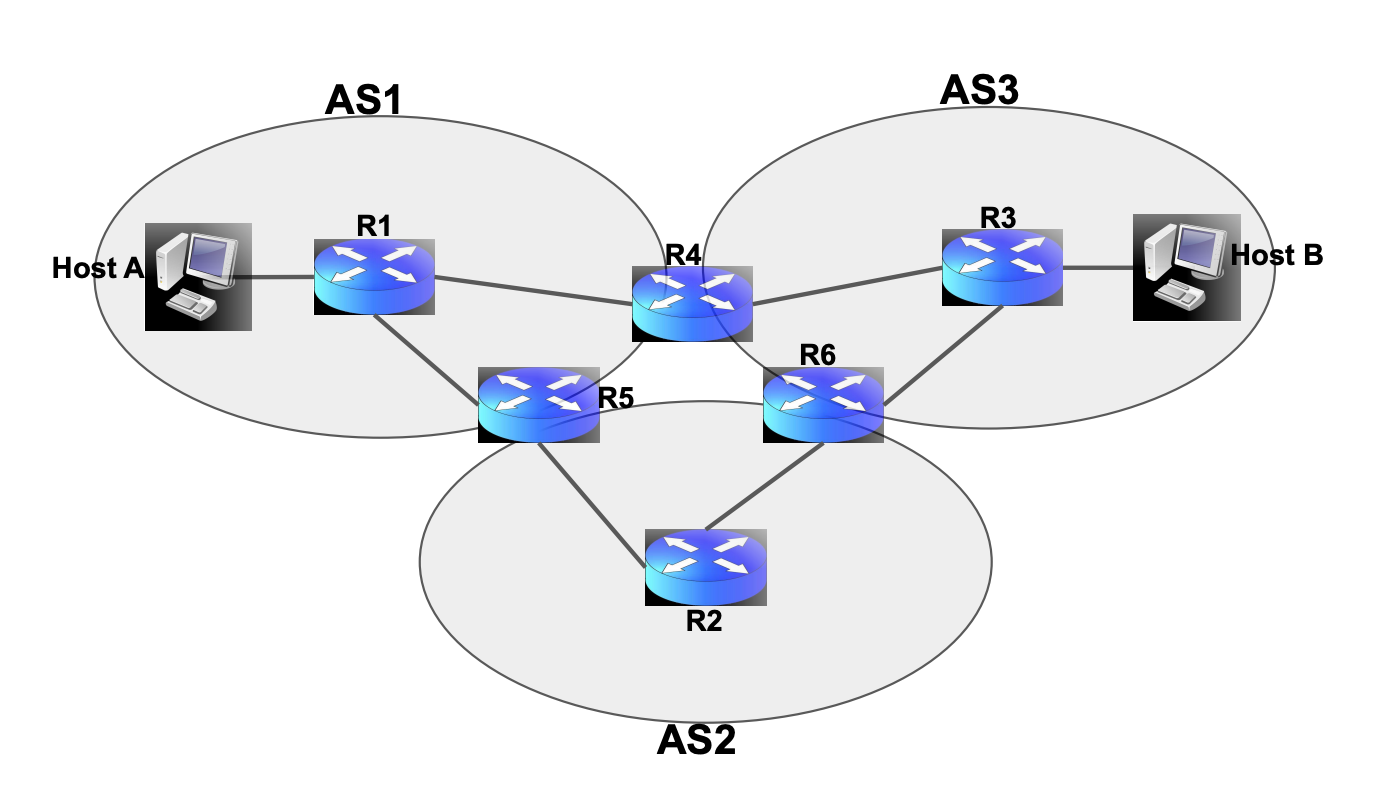
\includegraphics[scale=0.25]{q2.png}
        \caption{Sample topology.}
        \label{fig:q2.png}
    \end{center}
\end{figure}

%----------------------------------------------------------------------------------------------
% Q2.a
%----------------------------------------------------------------------------------------------
\begin{enumerate}
    \item
Please provide a list of routing protocols (or protocol families) that are at least required for each
router such that every router can obtain a route to all devices (i.e., hosts or routers). Assume
that there are no static routes. Justify your answer.
\end{enumerate}

\begin{tcolorbox}
    \mysolution{} 
    Here's a list of routing protocols that are required for routers in the network such that 
    every router can obtain a route to all devices. 
    \begin{itemize}
        \item Intra-AS routing protocol for AS1
        \item Intra-AS routing protocol for AS2
        \item Intra-AS routing protocol for AS3
        \item Inter-AS routing protocol
    \end{itemize}
\end{tcolorbox}

%----------------------------------------------------------------------------------------------
% Q2.b
%----------------------------------------------------------------------------------------------
\begin{enumerate}
    \setcounter{enumi}{1}
    \item
    Suppose Host A wants to communicate with Host B. Despite the potentially longer AS Path,
AS1 wants AS3 to route traffic via AS2. List three different ways in which AS1 might achieve
that goal. In addition, provide three different reasons why AS 1 might have chosen this policy.
\end{enumerate}

\begin{tcolorbox}
    \mysolution{} \\
    \begin{itemize}
        \item The capacity of the link that connects AS1 and AS3 directly might be not sufficient
            to handle all packets from AS1 to AS3 and vice versa. 
        \item It might be the case that direct connection between AS1 and AS3 has more number of
            intermediate routers than a path which goes through AS2. 
        \item AS2 might apply some security policies to packets, such that DDoS attacks are 
            prevented. 
    \end{itemize}
\end{tcolorbox}

%----------------------------------------------------------------------------------------------
% Q2.c
%----------------------------------------------------------------------------------------------
\begin{enumerate}
    \setcounter{enumi}{2}
    \item
    Do host A and host B need to speak BGP? Why/Why not?
\end{enumerate}

\begin{tcolorbox}
    \mysolution{} \\
    No, there is no need for host A and host B to speak BGP. In fact these hosts send their 
    packet to the first router they are connected to and these router speak BGP in order
    to be able to steer packets in the right direction. 
\end{tcolorbox}


%----------------------------------------------------------------------------------------------
% Q2.d
%----------------------------------------------------------------------------------------------
\begin{enumerate}
    \setcounter{enumi}{3}
    \item
When running continiously pings for 5 minutes from Host B to Host A, AS3 noticed that RTTs
via the direct link between AS1 and AS3 are higher than RTTs observed when using the route
via AS2. Why may this happen? Provide, and explain, two different reasons. Do you expect
those reasons to have transient or long-lasting effects?
\end{enumerate}

\begin{tcolorbox}
    \mysolution{} \\
    \begin{itemize}
        \item The capacity of the link that connects AS1 and AS3 directly might be lower 
            comparing to the capacity of routers in the path from AS1 to AS2 and AS2 to AS3.
        \item It might be the case that direct connection between AS1 and AS3 has more number of
            intermediate routers than a path which goes through AS2. 
    \end{itemize}
\end{tcolorbox}




%    \bibliographystyle{acm}
%    \bibliography{ref}
\end{document}
